\documentclass[
	%sans,			% use sans-serif font
	%serif,			% use serif-font
	%mathsans,		% set mathtext to sans-serif
	%mathserif,		% set mathtext to serif
	%10pt,
	10pt,
	%12pt,
	t		% add text at the top border of slide
	%slidescentered,% center text on slide
	%draft,			% compile as draft version
	%handout,		% create handout file
	%notes,			% include nodes in slides
	%compress		% compress navigation bar
]{beamer}

\usetheme{lmtslides}
\usepackage{eso-pic}
%\usepackage[pdftex]{color}
\usepackage{times}
\usepackage[latin1]{inputenc}
%\usepackage[T1]{fontenc}
\usepackage[amssymb]{SIunits}
\usepackage{amsmath,amsfonts,amssymb,amsthm}
\usepackage{eurosym}
\usepackage{booktabs}
\usepackage{colortbl}
\usepackage{url}
\usepackage{animate}
\usepackage{graphics}
\usepackage{multimedia}

\graphicspath{{figures/}}

% SET LANGUAGE HERE! (Babel is already included and setup by this call.)
%\setlang{de}		% <- GERMAN
\setlang{en}		% <- ENGLISH

\newcommand{\norm}[1]{\left\lVert#1\right\rVert}

% MODIFY THESE ACCORDINGLY! ---
\title{Parallel Mesh Simplification with Adaptive Thresholding Based on Quadric Error Metrics}
\subtitle{Interdisciplinary project}
\type{Sf} % (M/B/D/S)(f/m): (Master/Bachelor/Diplom/Studienarbeit)(final/midterm)
\author{Wojciech Zielonka}
\email{wojciech.zielonka@tum.de}
\advisor{Prof. Dr.-Ing. Eckehard Steinbach}
\emailAdvisor{eckehard.steinbach@tum.de}
\supervisor{Michael Gerstmayr}
\emailSupervisor{micheal.gerstmayr@navvis.com}
\date{\today}
%------------------------------


%%%%%%%%%%%%%%%%%%%%%%%%%%
\begin{document}

\AddToShipoutPicture{\TitlePicture}
\maketitle
\ClearShipoutPicture
\AddToShipoutPicture{\BackgroundPicture}

\section{Agenda}
\centering
\begin{frame}
\frametitle{Agenda}
\begin{center}
\begin{enumerate}
\centering
\item Introduction
\item Basic Simplification Algorithm
\item Extended Simplification Algorithm
\item Parallel Simplification Algorithm
\item Comparison to Commercially Available Products
\end{enumerate}
\end{center}
\end{frame}

\section{Short Introduction}
\centering
\begin{frame}
\frametitle{Introduction}
\begin{center}
The project was completed in NavVis company a part of research on mesh reconstruction using dense point clouds from laser scanned environments.
\end{center}
\end{frame}

\section{Get From}
\begin{frame}
\frametitle{Original Mesh}
\begin{figure}[ht]
	\centering
    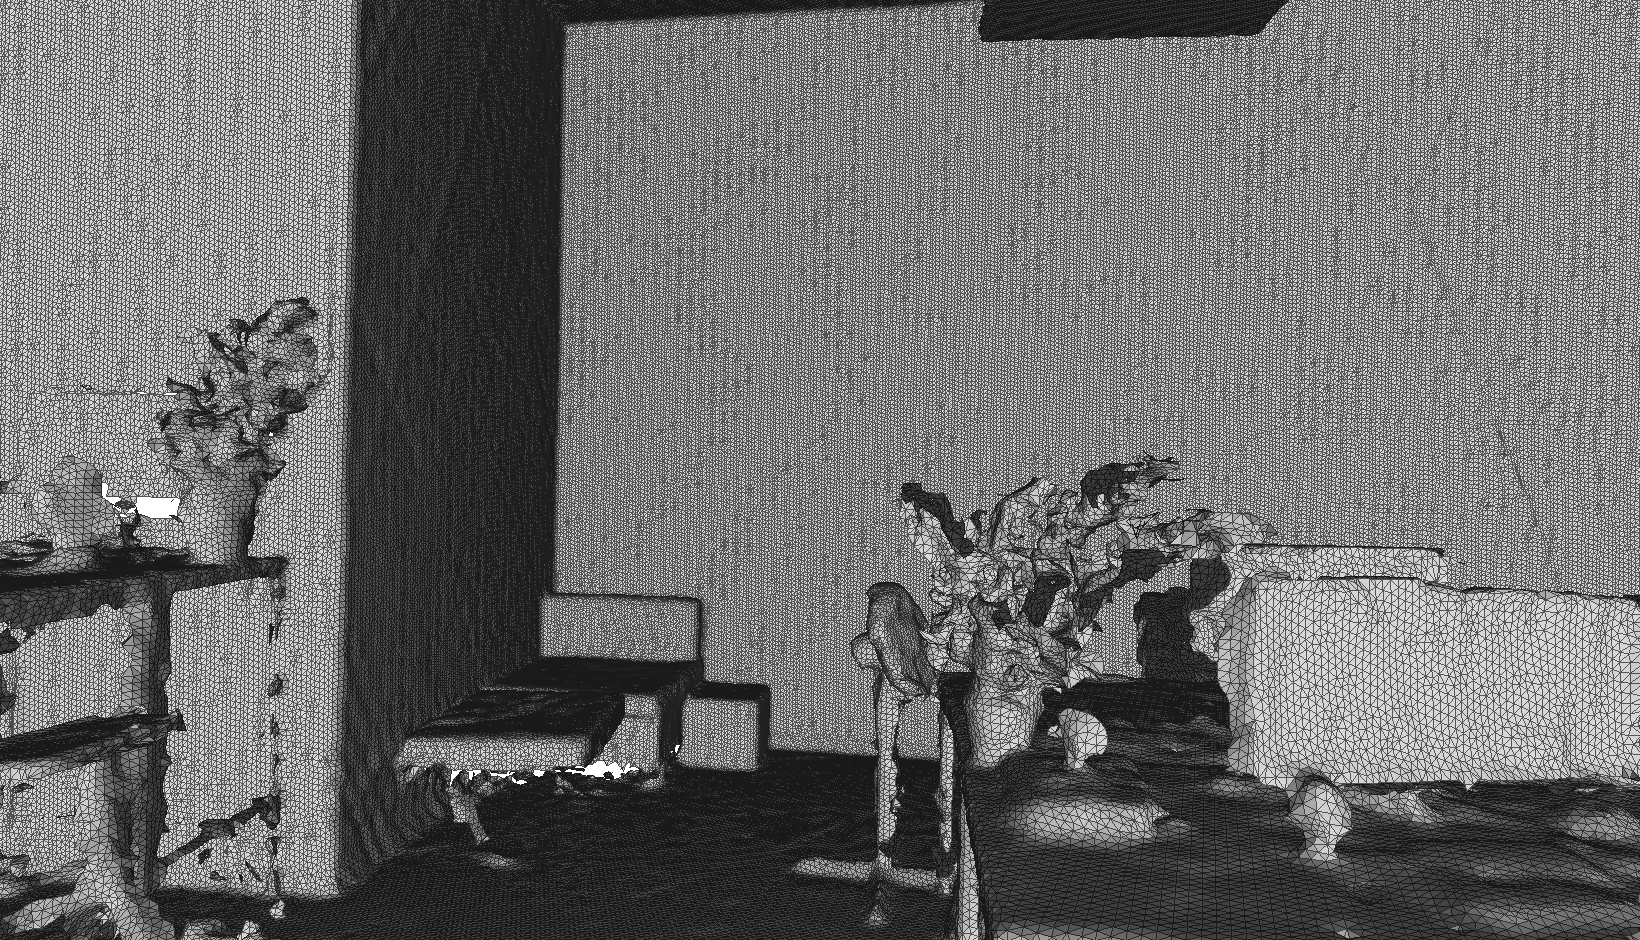
\includegraphics[width=1\textwidth]{from}
\end{figure}
\end{frame}

\section{Fast Edge Collapse [Geometry]}
\begin{frame}
\frametitle{Current Approach}
\begin{figure}[ht]
\centering
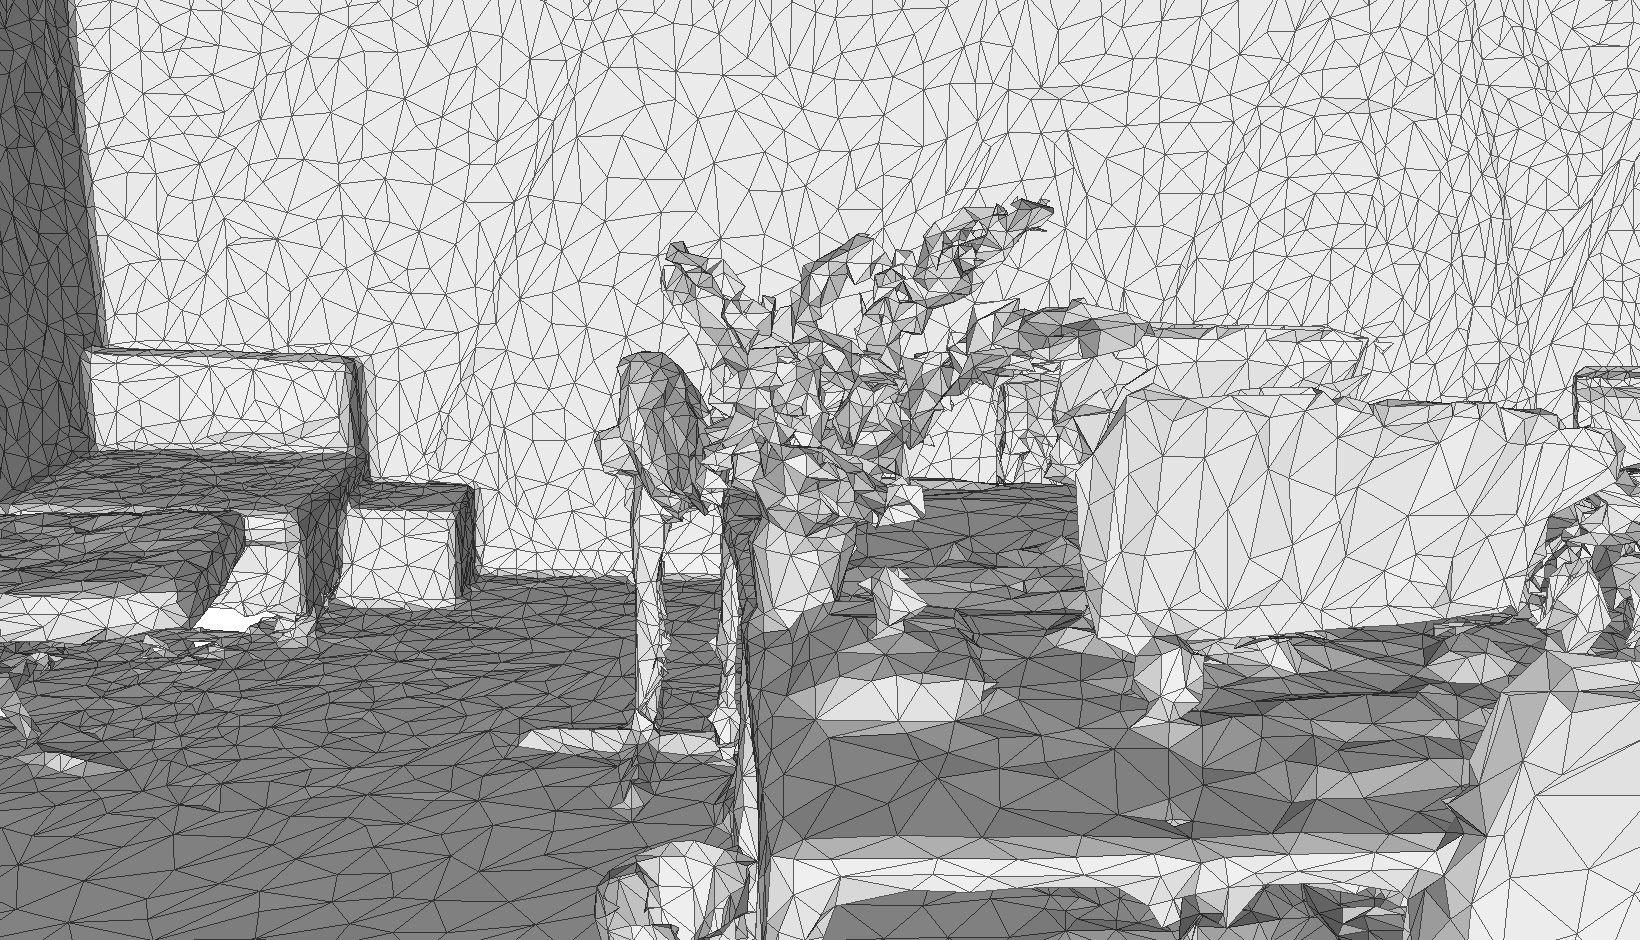
\includegraphics[width=1\textwidth]{fast_collapse}
\end{figure}
\end{frame}

\section{To}
\begin{frame}
\frametitle{This Work Approach}
\begin{figure}[ht]
	\centering
    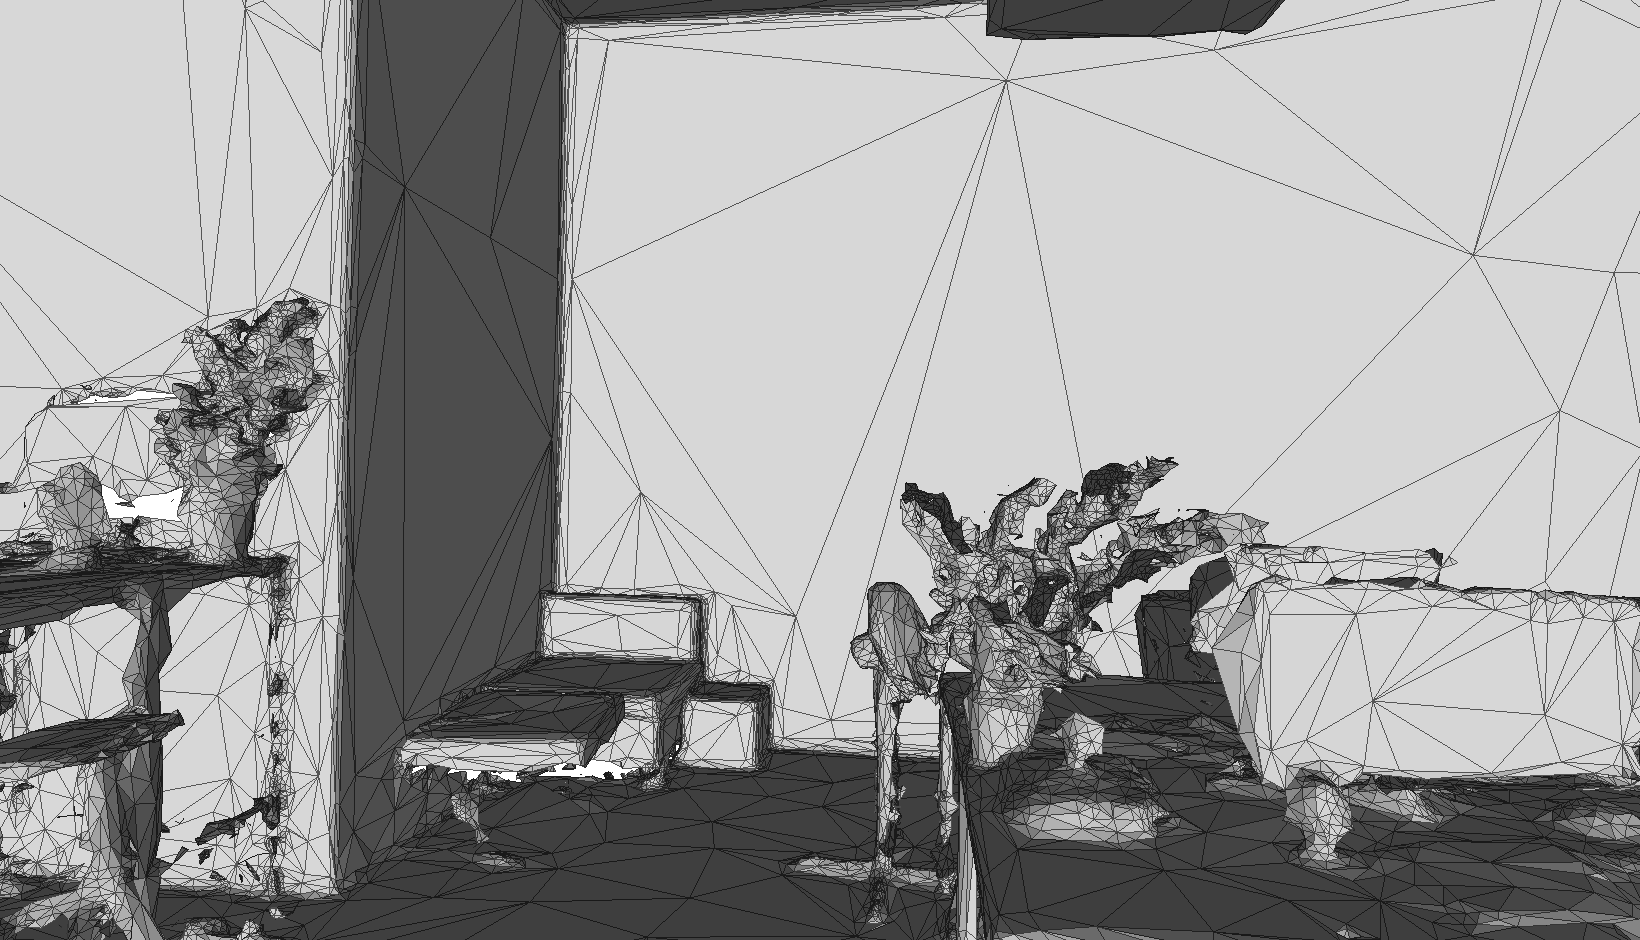
\includegraphics[width=1\textwidth]{to}
\end{figure}
\end{frame}

\section{Assumptions}
\begin{frame}
\frametitle{Goals}
\begin{enumerate}
\centering
\item Simplify mostly planar surface.
\item Preserve complex shapes as much as possible.
\item Use a parallel framework.
\end{enumerate}
\end{frame}

\section{What is a Decimation}
\begin{frame}
\frametitle{What is a Decimation?}
\begin{figure}[ht]
\centering
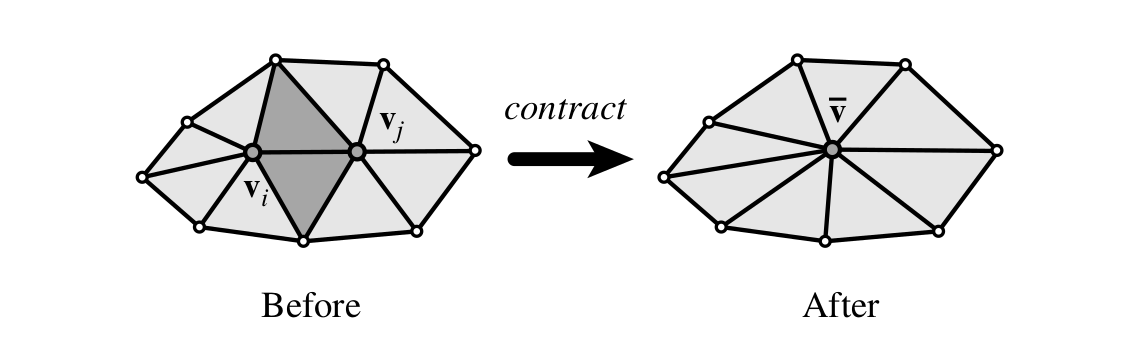
\includegraphics[width=1\textwidth]{edge_contraction}
\begin{align}
(\mathbf{v}_i, \mathbf{v}_j)\rightarrow\bar{\mathbf{v}}
\end{align}
\end{figure}
\end{frame}

\section{How to Select Edges?}
\begin{frame}
\frametitle{How to Select Edges?}
\centering
\begin{enumerate}
\item Select a set of candidate vertex pairs $(\mathbf{v_i}, \mathbf{v_j})$.
\item Allocate a quadric $Q_i$ for each vertex $\mathbf{v_i}$.
\item For each face compute a quadric $Q_i$. Add this quadric to the vertex quadrics $Q_i, Q_k, Q_l$ and optionally weight it appropriately.
\item For each candidate pair $(\mathbf{v_i}, \mathbf{v_j})$:
\begin{enumerate}
\item Compute $Q = Q_i + Q_j$.
\item Select a target position $\mathbf{\bar{v}}$.
\item Apply consistency checks and penalties.
\item Place pair in heap keys on cost $Q(\mathbf{\bar{v}})$
\end{enumerate}
\item Repeat until the desired approximation is reached:
\begin{enumerate}
\item Remove the pair $(\mathbf{v_i}, \mathbf{v_j})$ of least cost from the heap.
\item Preform contraction $(\mathbf{v_i}, \mathbf{v_j})\rightarrow\bar{\mathbf{v}}$
\item Set $Q_i = Q_i + Q_j$.
\item For each remaining pair $(\mathbf{v_i}, \mathbf{v_j})$, compute target position and cost as in step 4; update heap.
\end{enumerate}
\end{enumerate}
\end{frame}

\section{Quadric}
\begin{frame}
\frametitle{What is Quadric?}
\centering
$\mathbf{n}^T\mathbf{v}+d=0$\\ normal $\mathbf{n} = [a\;b\;c]^T$\\ $d$ is a scalar constant\\ $\mathbf{v} = [x\;y\;z]^T$ is a point in $3D$ space.
\\
\begin{align}
D^2(\mathbf{v}) &= (\mathbf{n}^T\mathbf{v}+d)^2 = (\mathbf{v}^T(\mathbf{n}\mathbf{n}^T)\mathbf{v}+2(d\mathbf{n})^T\mathbf{v}+d^2)\\
Q(\mathbf{v}) &= \mathbf{v}^T\mathbf{A}\mathbf{v} + 2\mathbf{b}^T\mathbf{v} + c\\
Q(\mathbf{v}) &= D^2(\mathbf{v})
\end{align}
\end{frame}

\section{How to Select Edges Quadric accumulation}
\begin{frame}
\frametitle{How to Select Edges?}
\centering
\begin{enumerate}
\color{gray}
\item Select a set of candidate vertex pairs $(\mathbf{v_i}, \mathbf{v_j})$.
\color{black}
\item Allocate a quadric $Q_i$ for each vertex $\mathbf{v_i}$.
\item For each face compute a quadric $Q_i$. Add this quadric to the vertex quadrics $Q_i, Q_k, Q_l$ and optionally weight it appropriately.
\color{gray}
\item For each candidate pair $(\mathbf{v_i}, \mathbf{v_j})$:
\color{gray}
\begin{enumerate}
\color{gray}
\item Compute $Q = Q_i + Q_j$.
\item Select a target position $\mathbf{\bar{v}}$.
\item Apply consistency checks and penalties.
\item Place pair in heap keys on cost $Q(\mathbf{\bar{v}})$
\end{enumerate}
\item Repeat until the desired approximation is reached:
\begin{enumerate}
\color{gray}
\item Remove the pair $(\mathbf{v_i}, \mathbf{v_j})$ of least cost from the heap.
\item Preform contraction $(\mathbf{v_i}, \mathbf{v_j})\rightarrow\bar{\mathbf{v}}$
\item Set $Q_i = Q_i + Q_j$.
\item For each remaining pair $(\mathbf{v_i}, \mathbf{v_j})$, compute target position and cost as in step 4; update heap.
\end{enumerate}
\end{enumerate}
\end{frame}

\section{Quadric Accumulation}
\begin{frame}
\frametitle{Quadric Accumulation}
\centering
\begin{enumerate}
\item [2.] Allocate a quadric $Q_i$ for each vertex $\mathbf{v_i}$.
\item [3.] For each face compute a quadric $Q_f$. Add this quadric to the vertex quadrics $Q_i, Q_k, Q_l$ and optionally weight it appropriately.
\end{enumerate}
\begin{align}
Q_i(\mathbf{v}) + Q_j(\mathbf{v}) &= (\mathbf{A_i} + \mathbf{A_j}, \mathbf{b_i} + \mathbf{b_j}, c_i + c_j)\\
E_Q(\mathbf{v}) &= \sum_{i} D_i^2(\mathbf{v}) = \sum_{i} Q_i(\mathbf{v}) = Q(\mathbf{v})
\end{align}
\end{frame}

\section{How to Select Edges Quadric accumulation}
\begin{frame}
\frametitle{How to Select Edges?}
\centering
\begin{enumerate}
\color{gray}
\item Select a set of candidate vertex pairs $(\mathbf{v_i}, \mathbf{v_j})$.
\item Allocate a quadric $Q_i$ for each vertex $\mathbf{v_i}$.
\item For each face compute a quadric $Q_i$. Add this quadric to the vertex quadrics $Q_i, Q_k, Q_l$ and optionally weight it appropriately.
\color{black}
\item For each candidate pair $(\mathbf{v_i}, \mathbf{v_j})$:
\color{gray}
\begin{enumerate}
\item Compute $Q = Q_i + Q_j$.
\item Select a target position $\mathbf{\bar{v}}$.
\item Apply consistency checks and penalties.
\item Place pair in heap keys on cost $Q(\mathbf{\bar{v}})$
\end{enumerate}
\color{gray}
\item Repeat until the desired approximation is reached:
\begin{enumerate}
\color{gray}
\item Remove the pair $(\mathbf{v_i}, \mathbf{v_j})$ of least cost from the heap.
\item Preform contraction $(\mathbf{v_i}, \mathbf{v_j})\rightarrow\bar{\mathbf{v}}$
\item Set $Q_i = Q_i + Q_j$.
\item For each remaining pair $(\mathbf{v_i}, \mathbf{v_j})$, compute target position and cost as in step 4; update heap.
\end{enumerate}
\end{enumerate}
\end{frame}

\section{Create Edges}
\begin{frame}
\frametitle{Create Edges}
\centering
\begin{enumerate}
\item [4.] For each candidate pair $(\mathbf{v_i}, \mathbf{v_j})$:
\begin{enumerate}
\item Compute $Q = Q_i + Q_j$.
\item Select a target position $\mathbf{\bar{v}}$.
\item Apply consistency checks and penalties.
\item Place pair in heap keys on cost $Q(\mathbf{\bar{v}})$
\end{enumerate}
\end{enumerate}

\begin{align}
Q(\mathbf{v}) &= \mathbf{v}^T\mathbf{A}\mathbf{v} + 2\mathbf{b}^T\mathbf{v} + c\\
\nabla Q(\mathbf{v}) &= 2\mathbf{A}\mathbf{v} + 2 \mathbf{b}
\end{align}
Solving for $\nabla Q(\mathbf{v}) = 0$, the optimal position is defined:
\begin{align}
\mathbf{\bar{v}} = -\mathbf{A}^{-1}\mathbf{b}
\label{v_bar}
\end{align}

\end{frame}

\section{How to Select Edges Quadric accumulation}
\begin{frame}
\frametitle{How to Select Edges?}
\centering
\begin{enumerate}
\color{gray}
\item Select a set of candidate vertex pairs $(\mathbf{v_i}, \mathbf{v_j})$.
\item Allocate a quadric $Q_i$ for each vertex $\mathbf{v_i}$.
\item For each face compute a quadric $Q_i$. Add this quadric to the vertex quadrics $Q_i, Q_k, Q_l$ and optionally weight it appropriately.
\item For each candidate pair $(\mathbf{v_i}, \mathbf{v_j})$:
\color{gray}
\begin{enumerate}
\color{gray}
\item Compute $Q = Q_i + Q_j$.
\item Select a target position $\mathbf{\bar{v}}$.
\item Apply consistency checks and penalties.
\item Place pair in heap keys on cost $Q(\mathbf{\bar{v}})$
\end{enumerate}
\color{black}
\item Repeat until the desired approximation is reached:
\begin{enumerate}
\item Remove the pair $(\mathbf{v_i}, \mathbf{v_j})$ of least cost from the heap.
\item Preform contraction $(\mathbf{v_i}, \mathbf{v_j})\rightarrow\bar{\mathbf{v}}$
\item Set $Q_i = Q_i + Q_j$.
\item For each remaining pair $(\mathbf{v_i}, \mathbf{v_j})$, compute target position and cost as in step 4; update heap.
\end{enumerate}
\end{enumerate}
\end{frame}

\section{Extended version with color and normals}
\begin{frame}
\frametitle{Extended Version With Color and Normals}
\centering
\begin{center}
To improve simplification more attributes are incorporated in the joint optimization. Using additionally, color and normals approximations are much closer to the desired goal.
\begin{align}
\mathbf{v} &= [x \ y \ z \ r \ g \ b]^T\\
T &= (\mathbf{p}, \mathbf{q}, \mathbf{r})\\ 
\mathbf{h} &= \mathbf{q} - \mathbf{p}\\
\mathbf{k} &= \mathbf{r} - \mathbf{p}
\end{align}
\end{center}
\end{frame}

\section{Plane}
\begin{frame}
\frametitle{Plane in $\mathbb{R}^n$}
\centering
\begin{align}
\mathbf{e_1} &= \mathbf{h} / \norm{\mathbf{h}} \\
\mathbf{e_2} &= \frac{\mathbf{k} - (\mathbf{e_1} \cdot \mathbf{k})\mathbf{e_1}}{\norm{\mathbf{k} - (\mathbf{e_1} \cdot \mathbf{k})\mathbf{e_1}}}
\end{align}
\begin{figure}[ht]
\centering
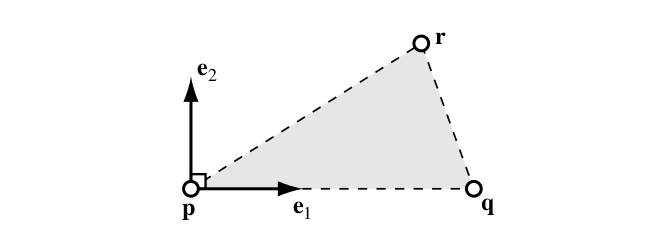
\includegraphics[width=0.8\textwidth]{gram}
\end{figure}
\end{frame}

\section{Extended version parameters}
\begin{frame}
\frametitle{Number of Parameters}
\centering
\begin{figure}[ht]
\centering
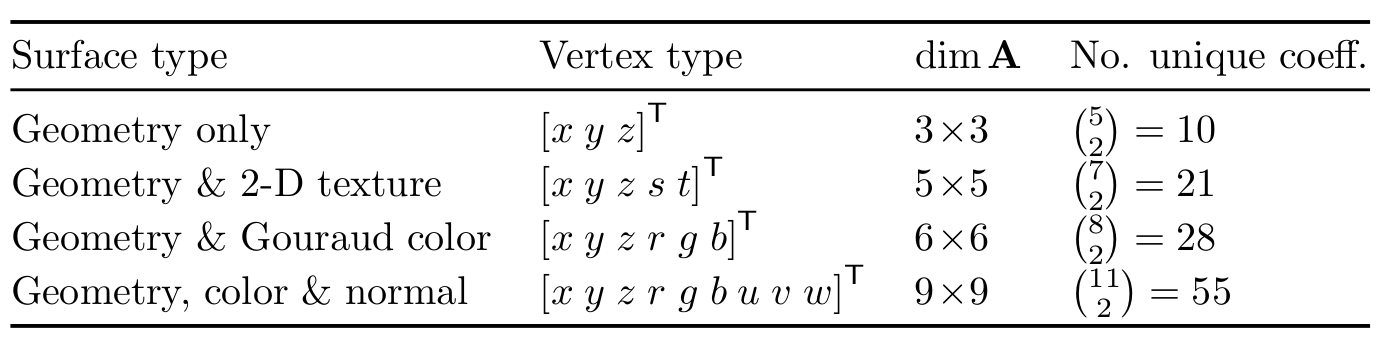
\includegraphics[width=1\textwidth]{params_table}
\end{figure}
\end{frame}

\section{Results}
\begin{frame}
\frametitle{Results}
\centering
\begin{figure}[ht]
\centering
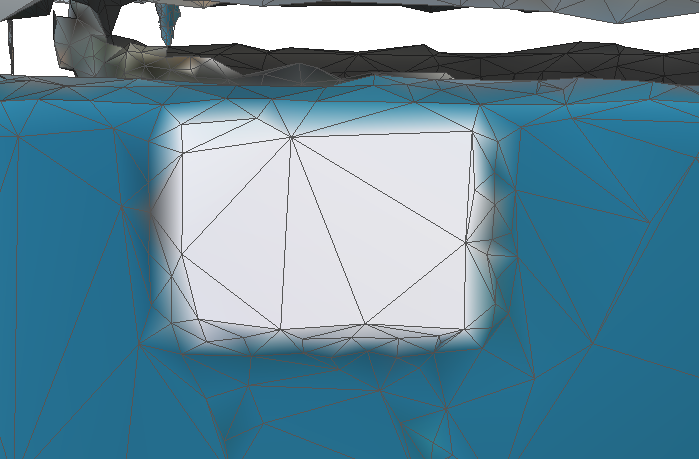
\includegraphics[width=10cm,height=6cm]{color_2}
\end{figure}
\end{frame}

\section{Results}
\begin{frame}
\frametitle{Results}
\centering
\begin{figure}[ht]
\centering
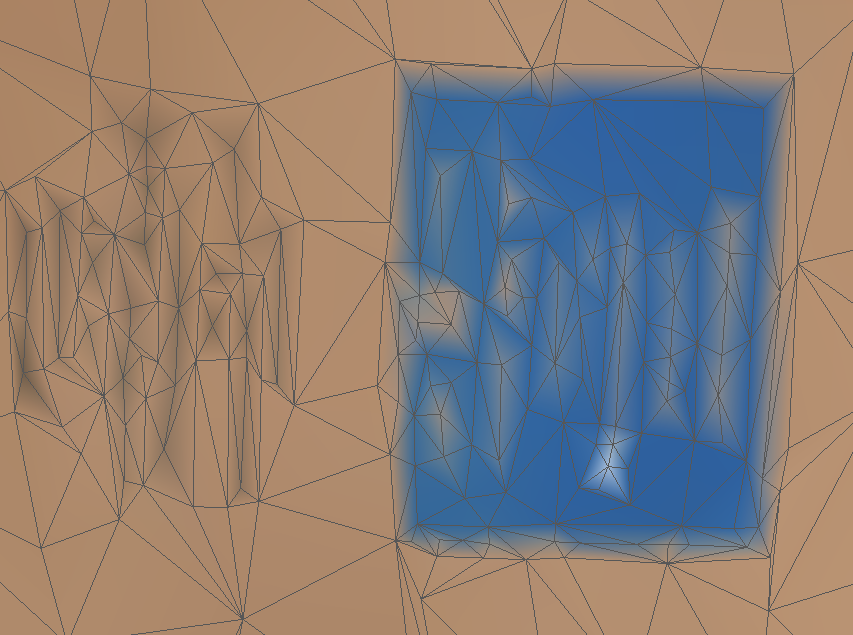
\includegraphics[width=10cm,height=6cm]{color_3}
\end{figure}
\end{frame}

\section{Results}
\begin{frame}
\frametitle{Results}
\centering
\begin{figure}[ht]
\centering
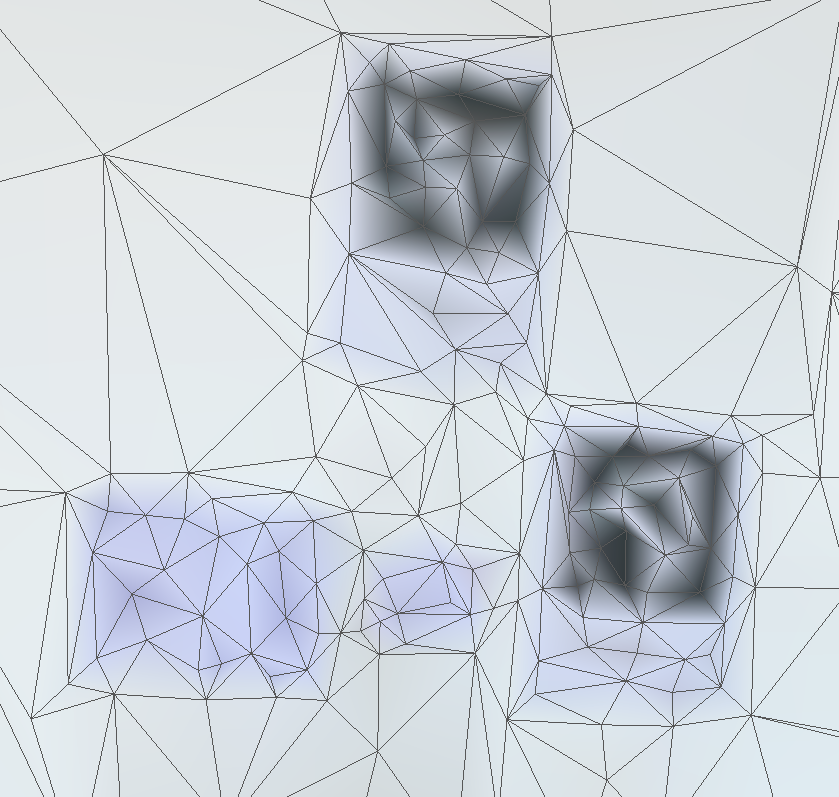
\includegraphics[width=10cm,height=6cm]{color_6}
\end{figure}
\end{frame}

\section{Results}
\begin{frame}
\frametitle{Results}
\centering
\begin{figure}[ht]
\centering
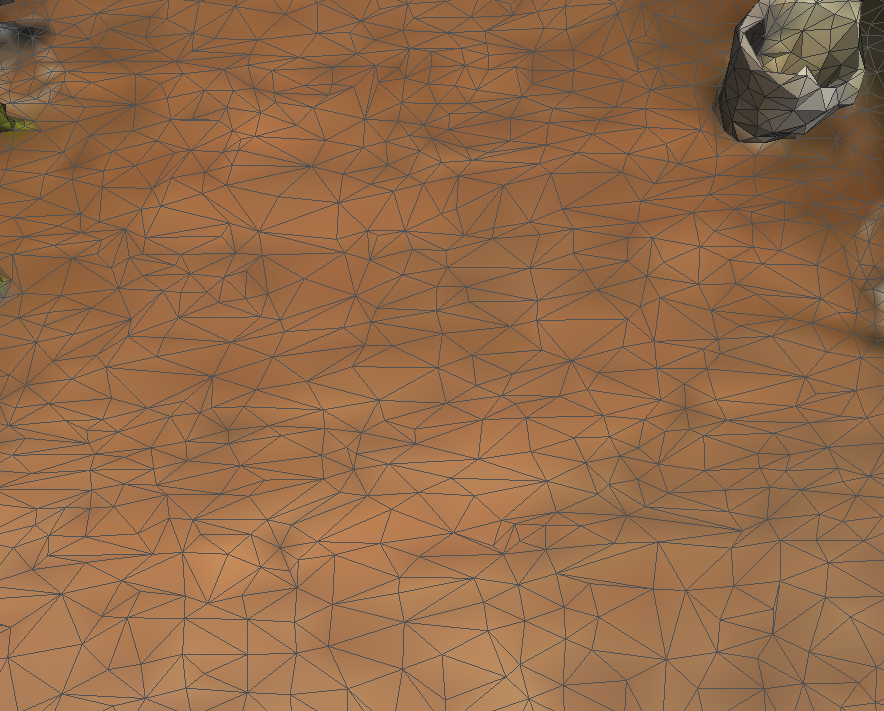
\includegraphics[width=10cm,height=6cm]{nosiy_floor}
\end{figure}
\end{frame}

\section{Results}
\begin{frame}
\frametitle{Results}
\centering
\begin{figure}[ht]
\centering
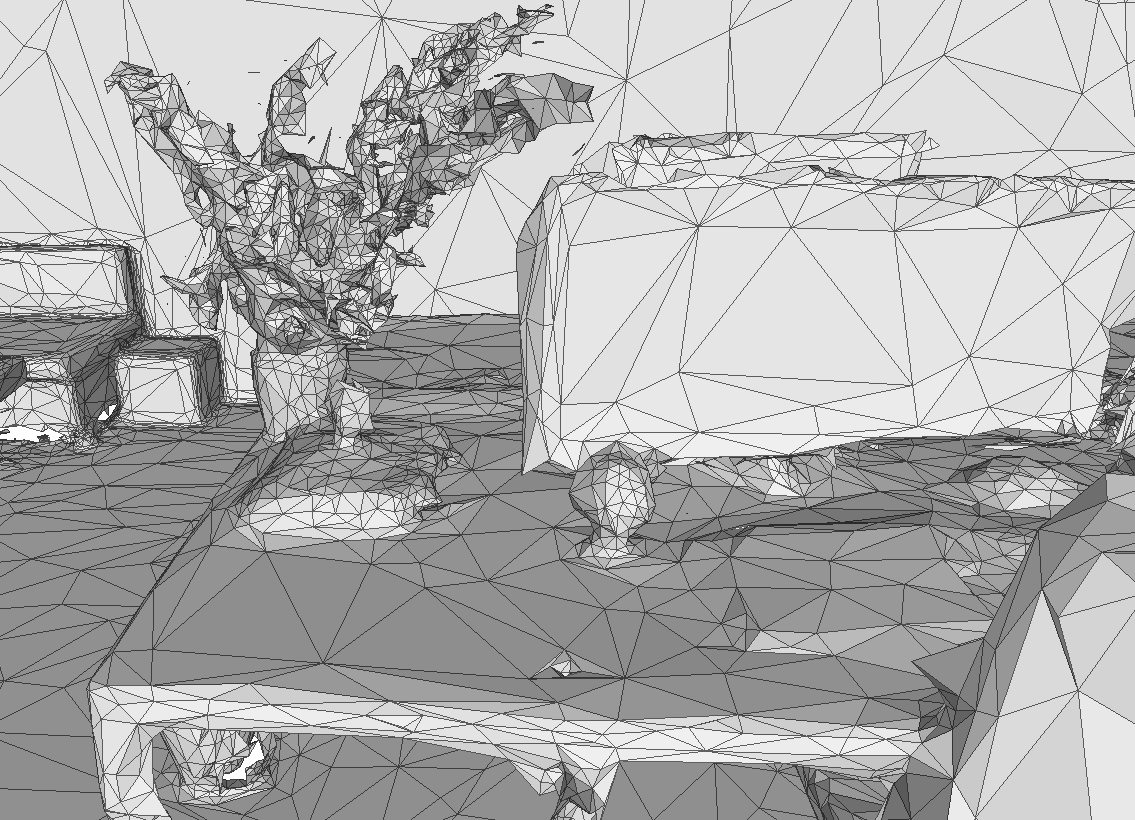
\includegraphics[width=10cm,height=6cm]{desk}
\end{figure}
\end{frame}

\section{Parallel Iterative Adaptive Thresholding}
\begin{frame}
\frametitle{Parallel Iterative Adaptive Thresholding}
\centering
\begin{enumerate}
\item Smooth mesh using Taubin's algorithm (optional).
\item Cluster the mesh:
\begin{enumerate}
\item Split the mesh according to number of selected clusters; for example 2x2x2=8.
\item Add a task for each cluster to the queue.
\end{enumerate}
\item Wait for all threads from the thread-pool to finish processing simplification algorithm [QSlim] ran on all clusters. Each thread does:
\begin{enumerate}
\item Build the heap with edges.
\item Decimate edges till reaching the threshold level.
\end{enumerate}
\item Update the mesh structure:
\begin{enumerate}
\item Remove faces flagged as invalid.
\item Reset properties for each remaining face and vertex.
\end{enumerate}
\item Repeat from the second step till convergence.
\end{enumerate}
\end{frame}

\section{Parallel Iterative Adaptive Thresholding}
\begin{frame}
\frametitle{Parallel Iterative Adaptive Thresholding}
\centering
\begin{enumerate}
\item Smooth mesh using Taubin's algorithm (optional).
\color{gray}
\item Cluster the mesh:
\begin{enumerate}
\color{gray}
\item Split the mesh according to number of selected clusters; for example 2x2x2=8.
\item Add a task for each cluster to the queue.
\end{enumerate}
\item Wait for all threads from the thread-pool to finish processing simplification algorithm [QSlim] ran on all clusters. Each thread does:
\begin{enumerate}
\color{gray}
\item Build the heap with edges.
\item Decimate edges till reaching the threshold level.
\end{enumerate}
\item Update the mesh structure:
\begin{enumerate}
\color{gray}
\item Remove faces flagged as invalid.
\item Reset properties for each remaining face and vertex.
\end{enumerate}
\item Repeat from the second step till convergence.
\end{enumerate}
\end{frame}

\section{Smoothing}
\begin{frame}
\frametitle{Taubin's algorithm}
\centering
\begin{enumerate}
\item [1.] Smooth mesh using Taubin's algorithm (optional).
\end{enumerate}
Taubin Smoothing is a linear low-pass filter that removes high curvature variations and does not produce shrinkage.
\begin{figure}[ht]
\centering
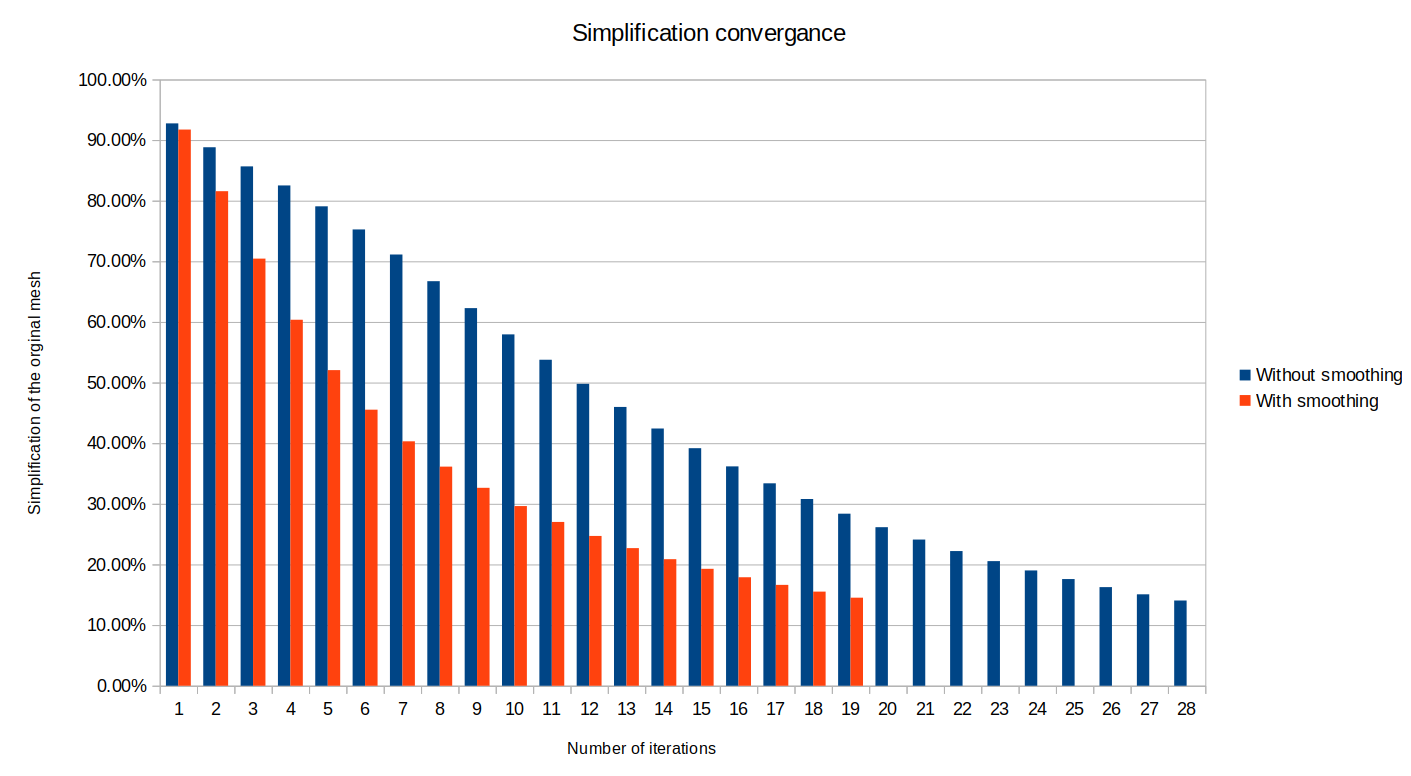
\includegraphics[width=0.8\textwidth]{convergance}
\end{figure}
\end{frame}

\section{Parallel Iterative Adaptive Thresholding}
\begin{frame}
\frametitle{Parallel Iterative Adaptive Thresholding}
\centering
\begin{enumerate}
\color{gray}
\item Smooth mesh using Taubin's algorithm (optional).
\color{black}
\item Cluster the mesh:
\begin{enumerate}
\item Split the mesh according to number of selected clusters; for example 2x2x2=8.
\item Add a task for each cluster to the queue.
\end{enumerate}
\color{gray}
\item Wait for all threads from the thread-pool to finish processing simplification algorithm [QSlim] ran on all clusters. Each thread does:
\begin{enumerate}
\color{gray}
\item Build the heap with edges.
\item Decimate edges till reaching the threshold level.
\end{enumerate}
\item Update the mesh structure:
\begin{enumerate}
\color{gray}
\item Remove faces flagged as invalid.
\item Reset properties for each remaining face and vertex.
\end{enumerate}
\item Repeat from the second step till convergence.
\end{enumerate}
\end{frame}

\section{Clustering}
\begin{frame}
\frametitle{Mesh Clustering}
\begin{enumerate}
\item [2.] Cluster the mesh:
\begin{enumerate}
\item Split the mesh according to number of selected clusters; for example 2x2x2=8.
\item Add a task for each cluster to the queue.
\end{enumerate}
\end{enumerate}
\begin{figure}[ht]
\centering
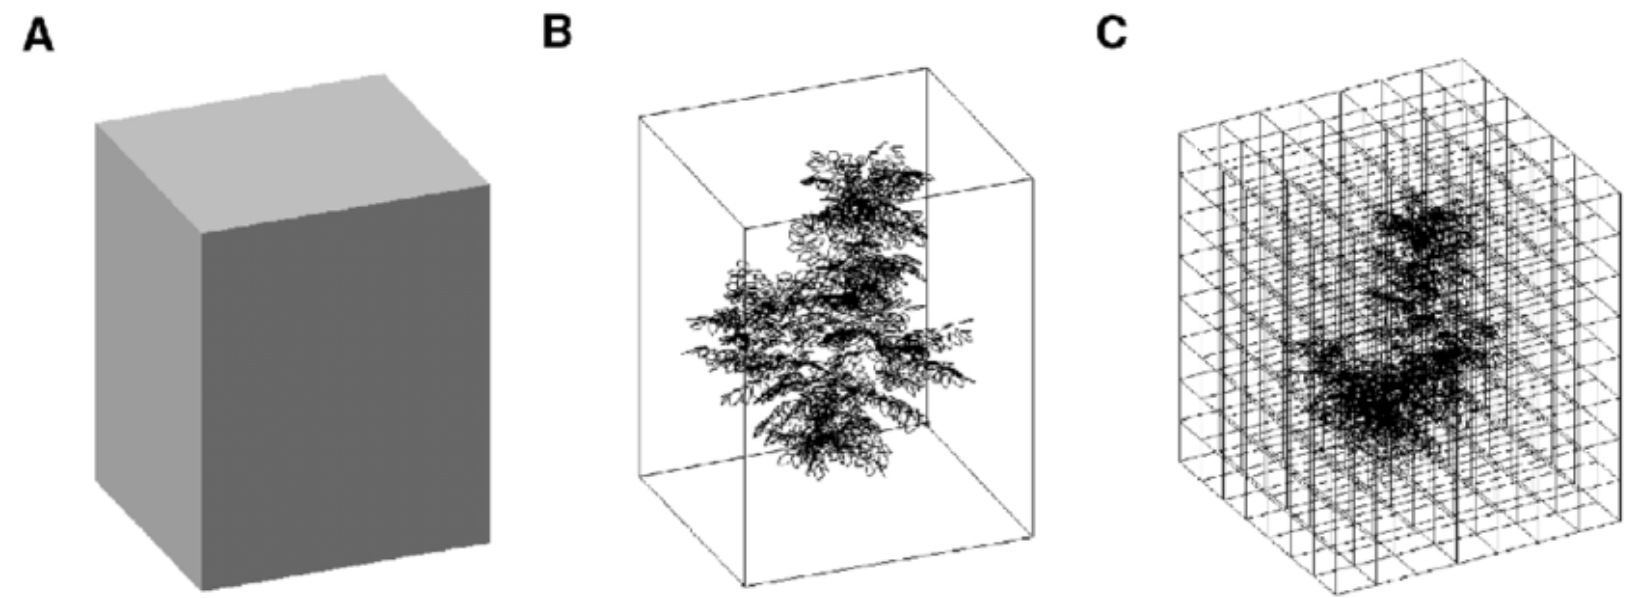
\includegraphics[width=0.8\textwidth]{clustering}
\end{figure}
\end{frame}

\section{Parallel Iterative Adaptive Thresholding}
\begin{frame}
\frametitle{Parallel Iterative Adaptive Thresholding}
\centering
\begin{enumerate}
\color{gray}
\item Smooth mesh using Taubin's algorithm (optional).
\item Cluster the mesh:
\begin{enumerate}
\color{gray}
\item Split the mesh according to number of selected clusters; for example 2x2x2=8.
\item Add a task for each cluster to the queue.
\end{enumerate}
\color{black}
\item Wait for all threads from the thread-pool to finish processing simplification algorithm [QSlim] ran on all clusters. Each thread does:
\begin{enumerate}
\item Build the heap with edges.
\item Decimate edges till reaching the threshold level.
\end{enumerate}
\item Update the mesh structure:
\begin{enumerate}
\item Remove faces flagged as invalid.
\item Reset properties for each remaining face and vertex.
\end{enumerate}
\item Repeat from the second step till convergence.
\end{enumerate}
\end{frame}

\section{Producer Consumer}
\begin{frame}
\frametitle{Producer Consumer Design Pattern}
\begin{figure}[ht]
\centering
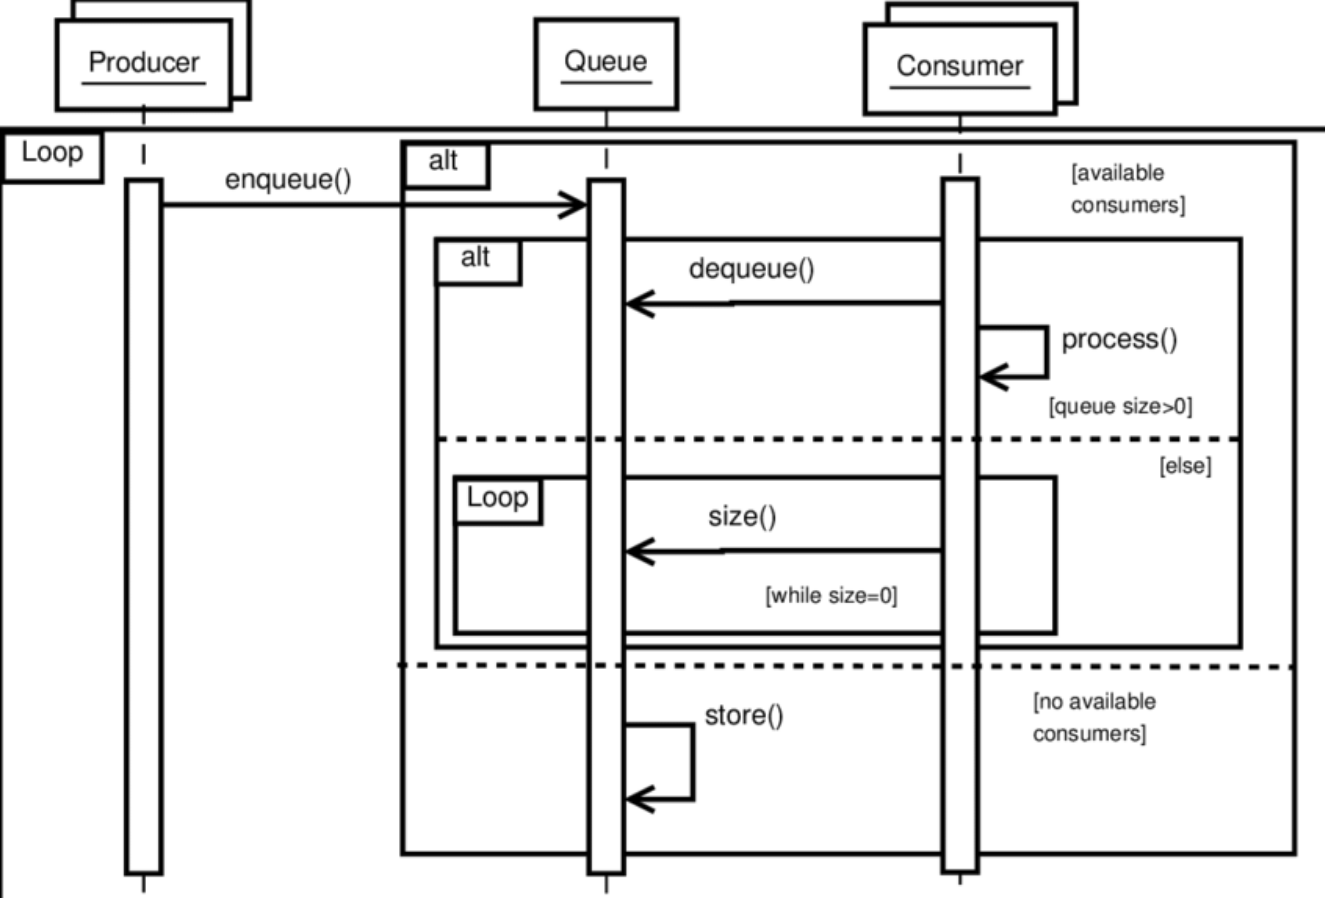
\includegraphics[width=0.8\textwidth]{producer_consumer}
\end{figure}
\end{frame}

\section{Parallel speedup}
\begin{frame}
\centering
\frametitle{Parallel speedup}
The tests were performed on a machine with 32 GB of RAM and Intel i7-6700 CPU 3.40GHz with 4 physical cores on a mesh with 982624 faces and 517715 vertices. Six different setups were ran with the objective to achieve reduction level 85\% of the original mesh.
\begin{table}[h!]
\centering
\begin{tabular}{ |c|c|c| } 
 \hline
 Number of clusters & Threads in the pool & Total time processing\\
 \hline
 1 & 1 & 127.62s\\
 8 & 2 & 77.98s\\
 8 & 4 & 56.77s\\
 8 & 8 & 62.01s\\
 27 & 8 & 48.88s\\
 27 & 27 & 48.02s\\
 \hline
\end{tabular}
\caption{4 different test setups.}
\end{table}
\end{frame}

\section{Results}
\begin{frame}
\frametitle{Results}
\begin{figure}[ht]
\centering
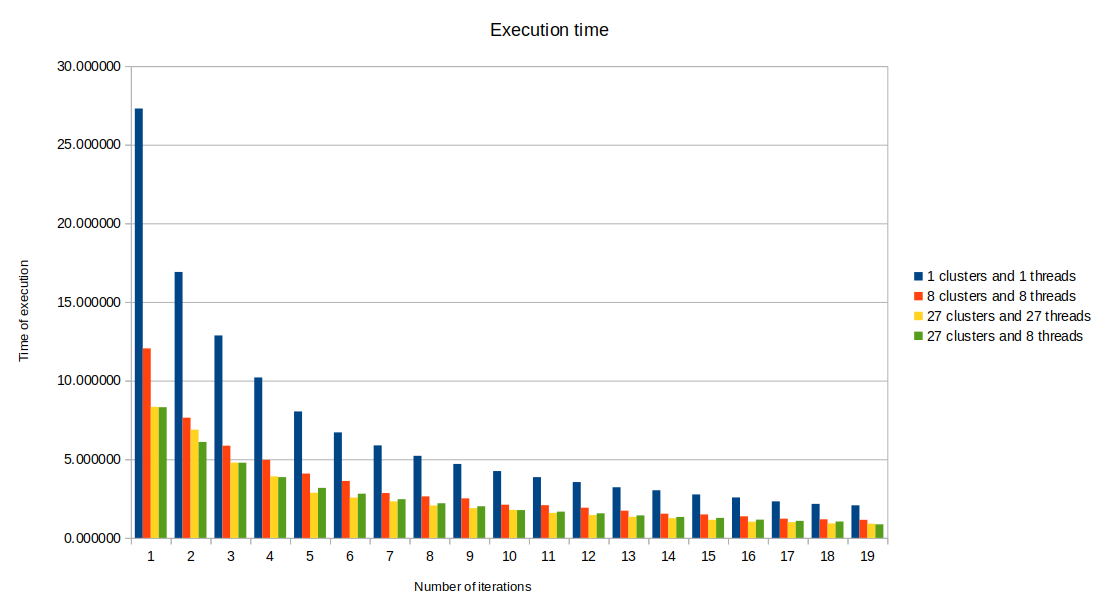
\includegraphics[width=1\textwidth]{chart}
\end{figure}
\end{frame}

\section{Speedup per iteration}
\begin{frame}
\frametitle{Speedup per iteration}
\begin{figure}[ht]
\centering
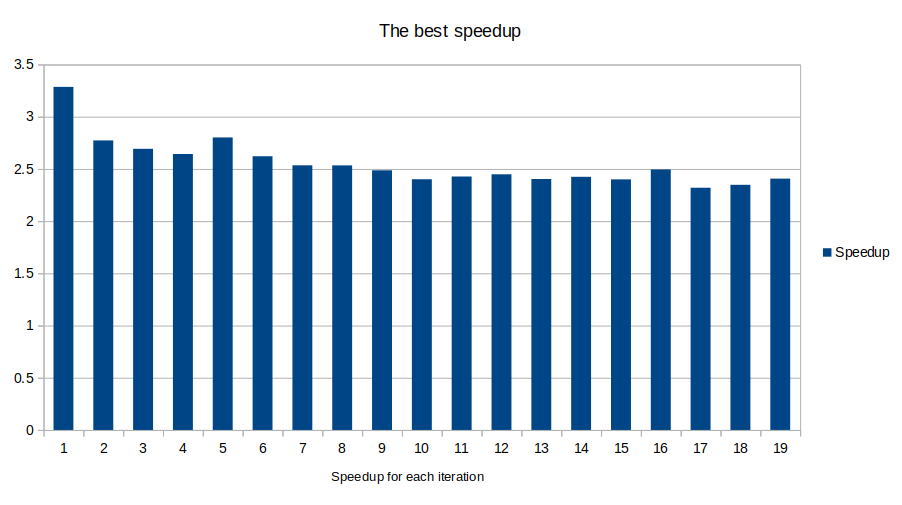
\includegraphics[width=1\textwidth]{chart2}
\end{figure}
\end{frame}

\section{Comparison to Commercially Available Products}
\begin{frame}
\frametitle{Comparison to Commercially Available Products}
\begin{figure}[ht]
\centering
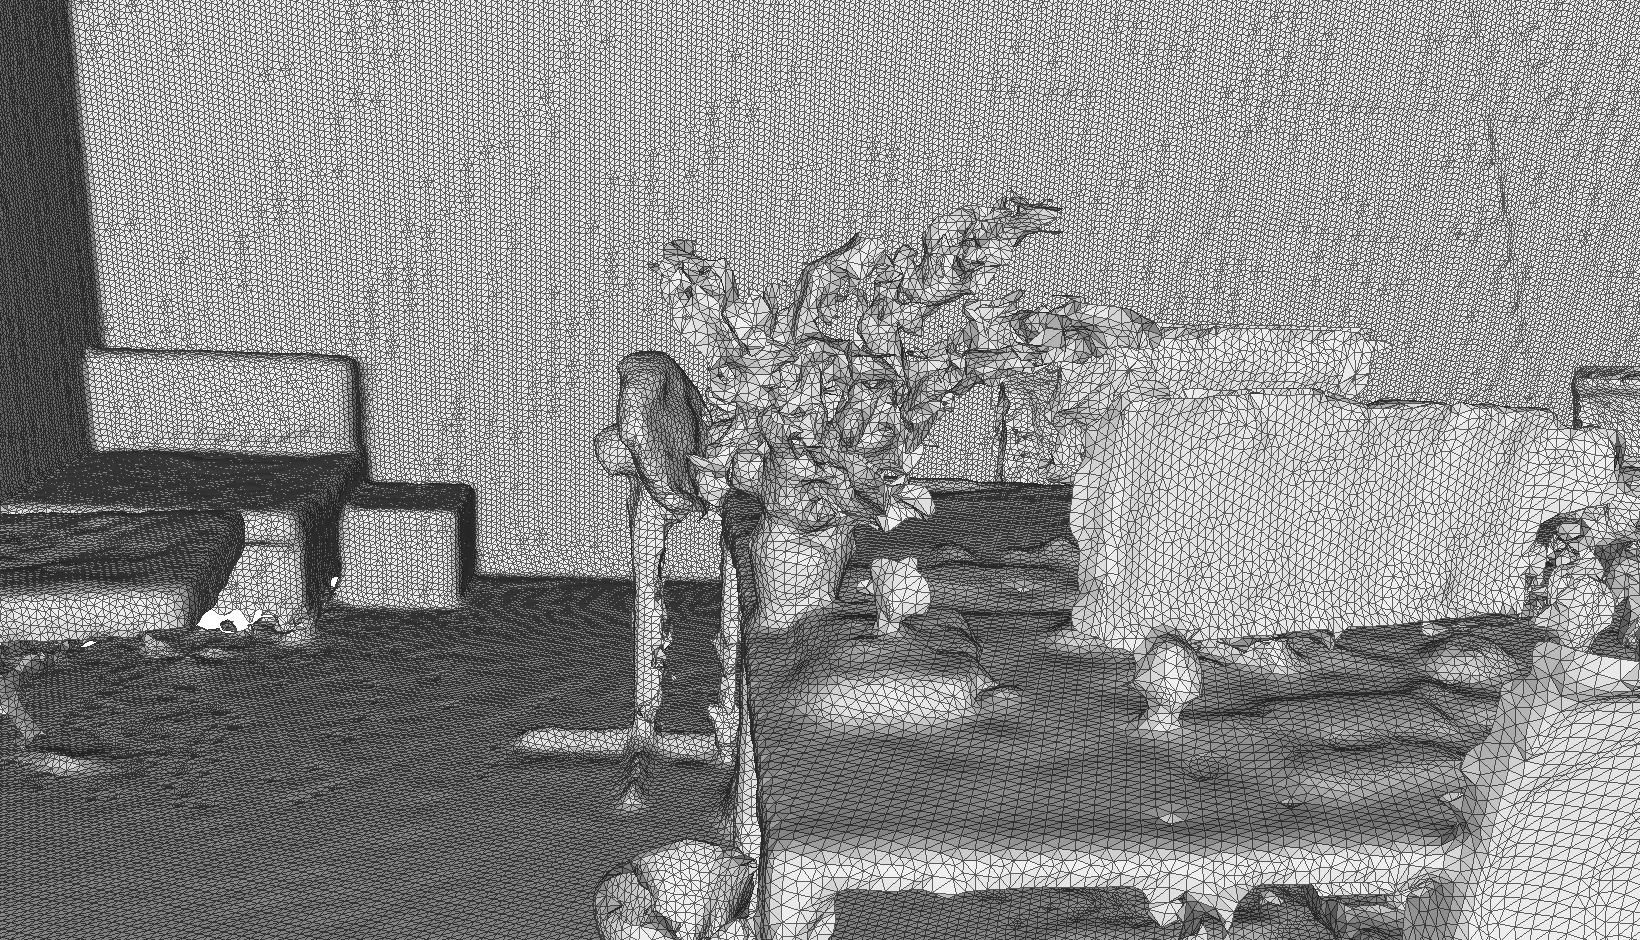
\includegraphics[width=1\textwidth]{original}
\end{figure}
\end{frame}

\section{Fast Edge Collapse [Geometry]}
\begin{frame}
\frametitle{Fast Edge Collapse [Geometry]}
\begin{figure}[ht]
\centering
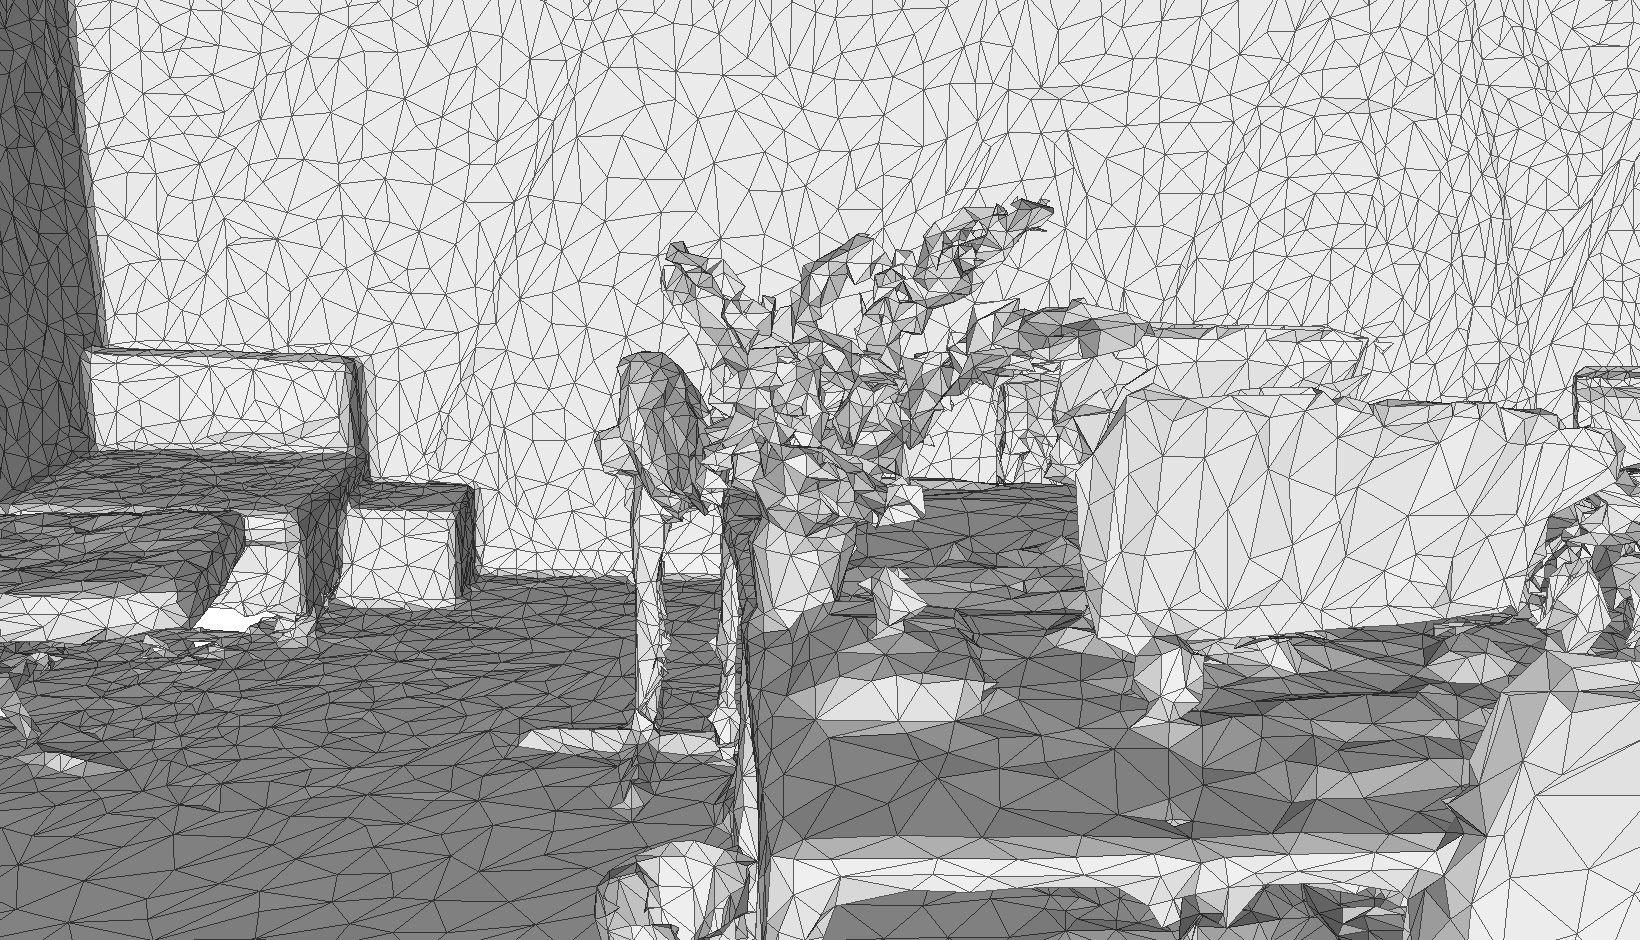
\includegraphics[width=1\textwidth]{fast_collapse}
\end{figure}
\end{frame}

\section{OpenMesh [Geometry, Normals]}
\begin{frame}
\frametitle{OpenMesh [Geometry, Normals]}
\begin{figure}[ht]
\centering
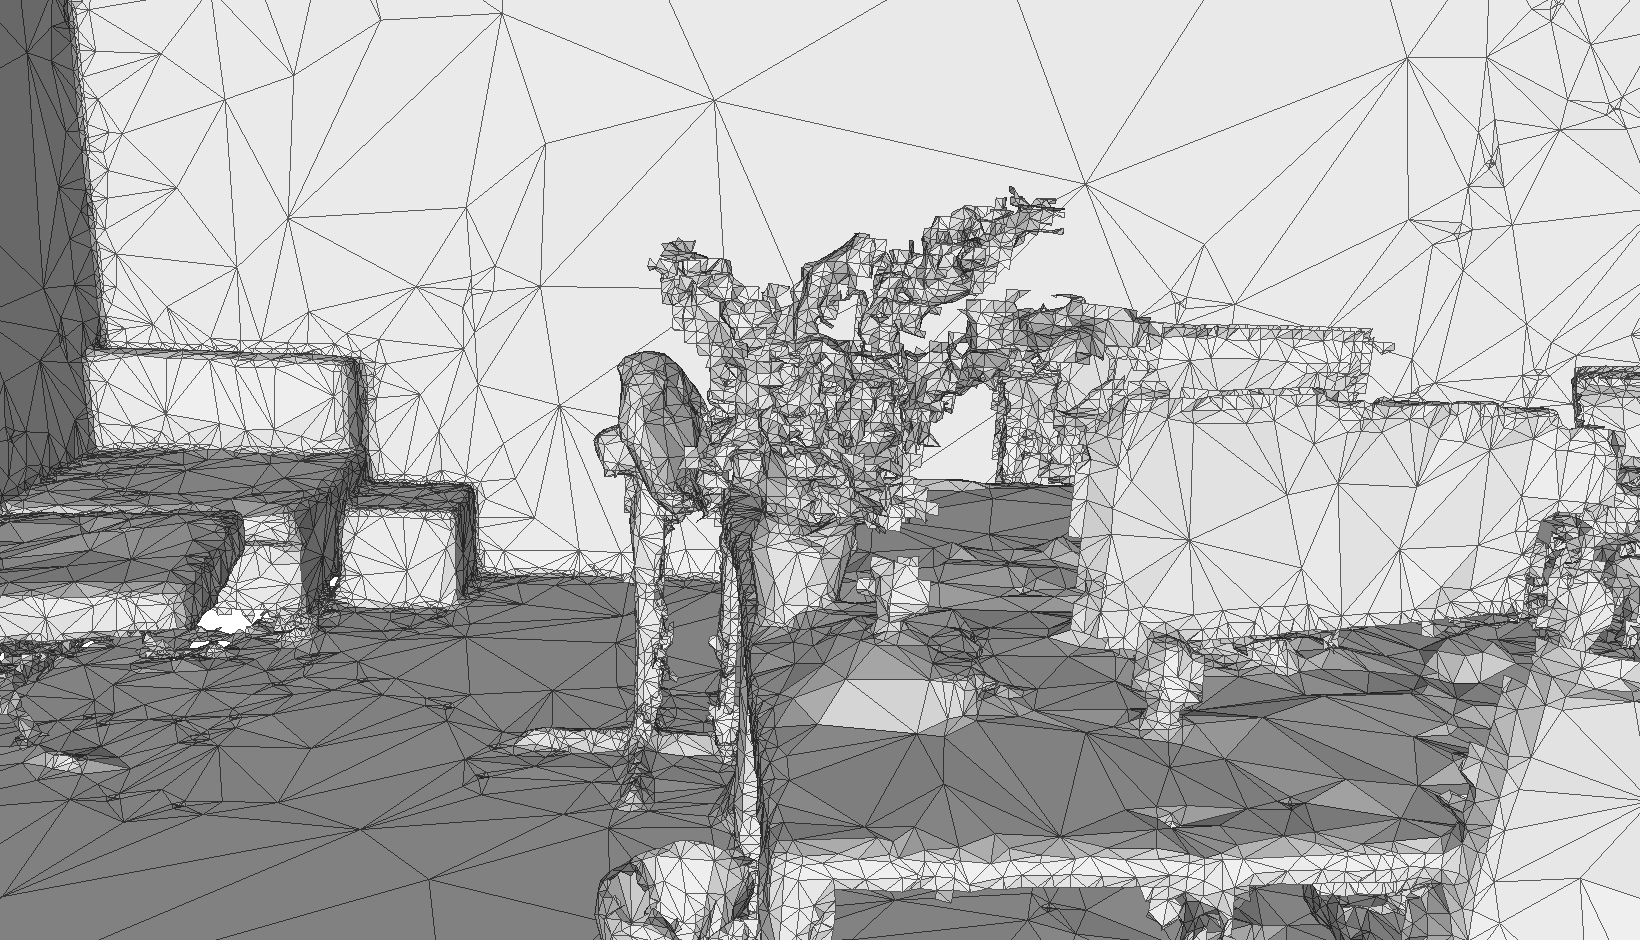
\includegraphics[width=1\textwidth]{open_mesh}
\end{figure}
\end{frame}

\section{Parallel QSlim [Geometry]}
\begin{frame}
\frametitle{Parallel QSlim [Geometry]}
\begin{figure}[ht]
\centering
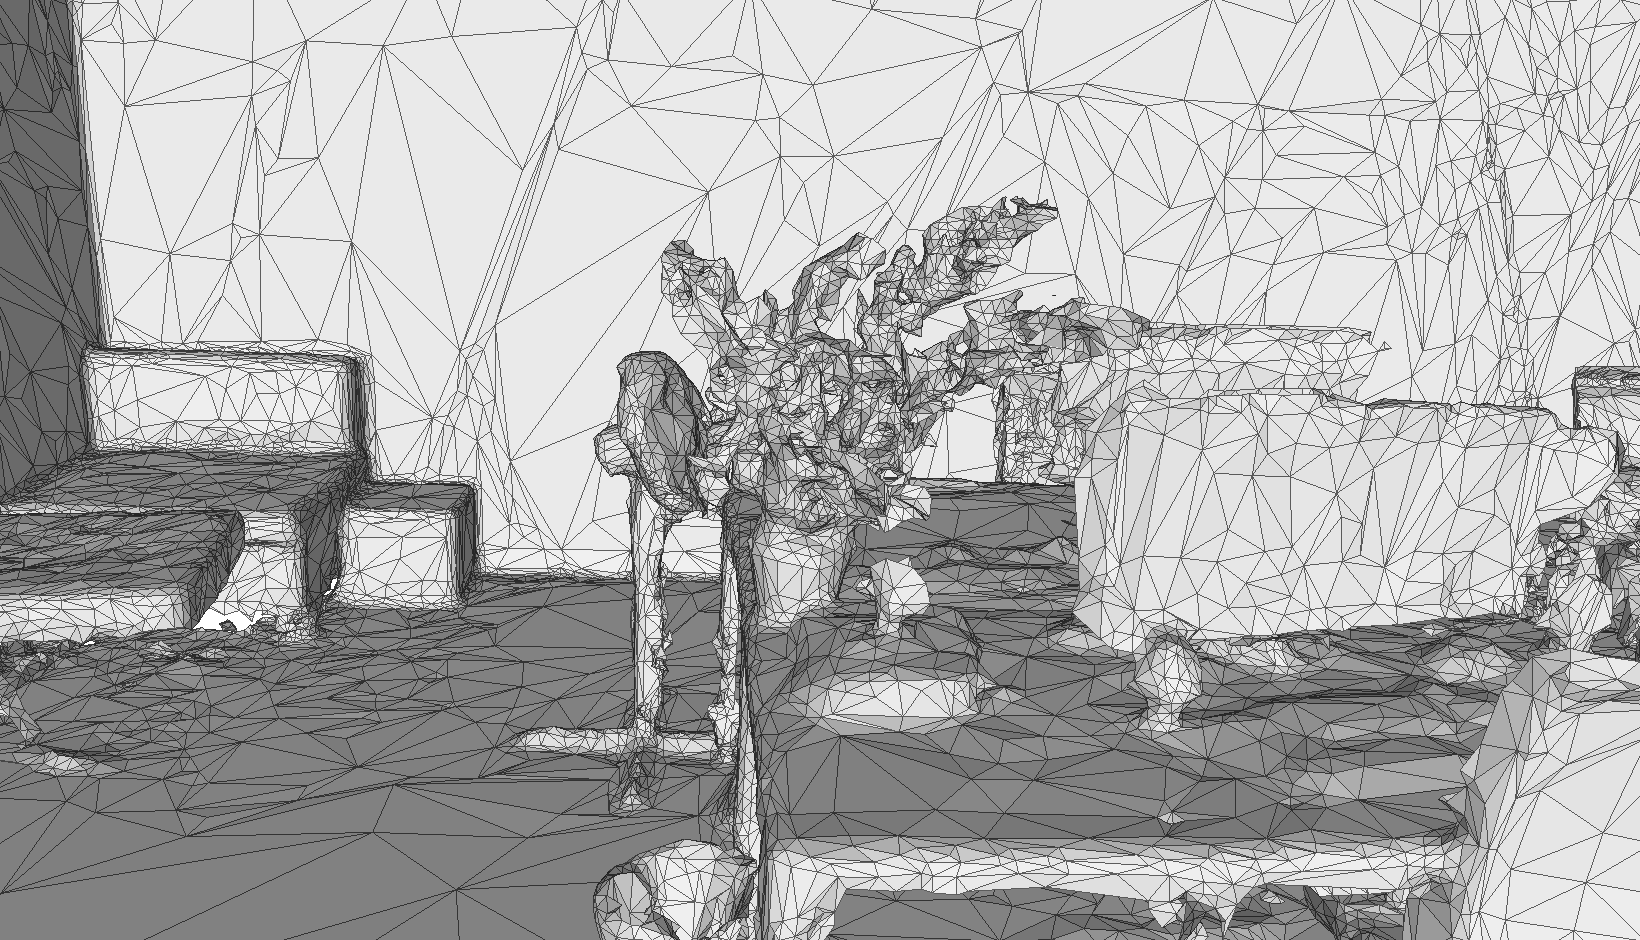
\includegraphics[width=1\textwidth]{my_3}
\end{figure}
\end{frame}

\section{Parallel QSlim [Geometry, Normals, Color]}
\begin{frame}
\frametitle{Parallel QSlim [Geometry, Normals, Color]}
\begin{figure}[ht]
\centering
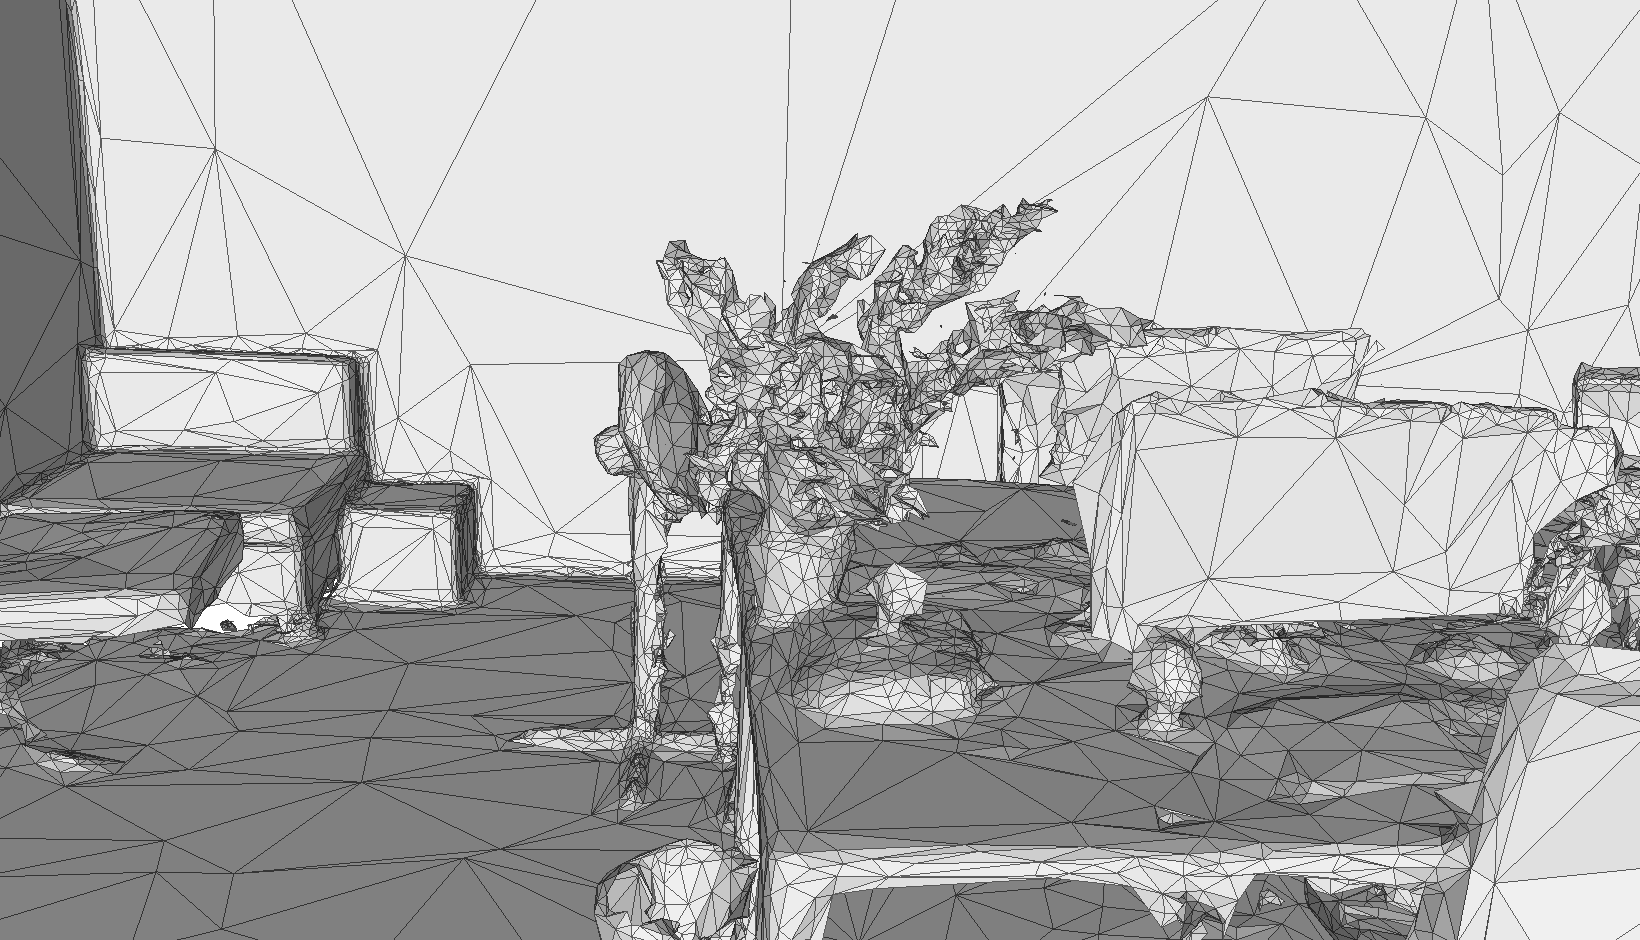
\includegraphics[width=1\textwidth]{my_9}
\end{figure}
\end{frame}

\section{RapidCompact [Geometry]}
\begin{frame}
\frametitle{RapidCompact [Geometry]}
\begin{figure}[ht]
\centering
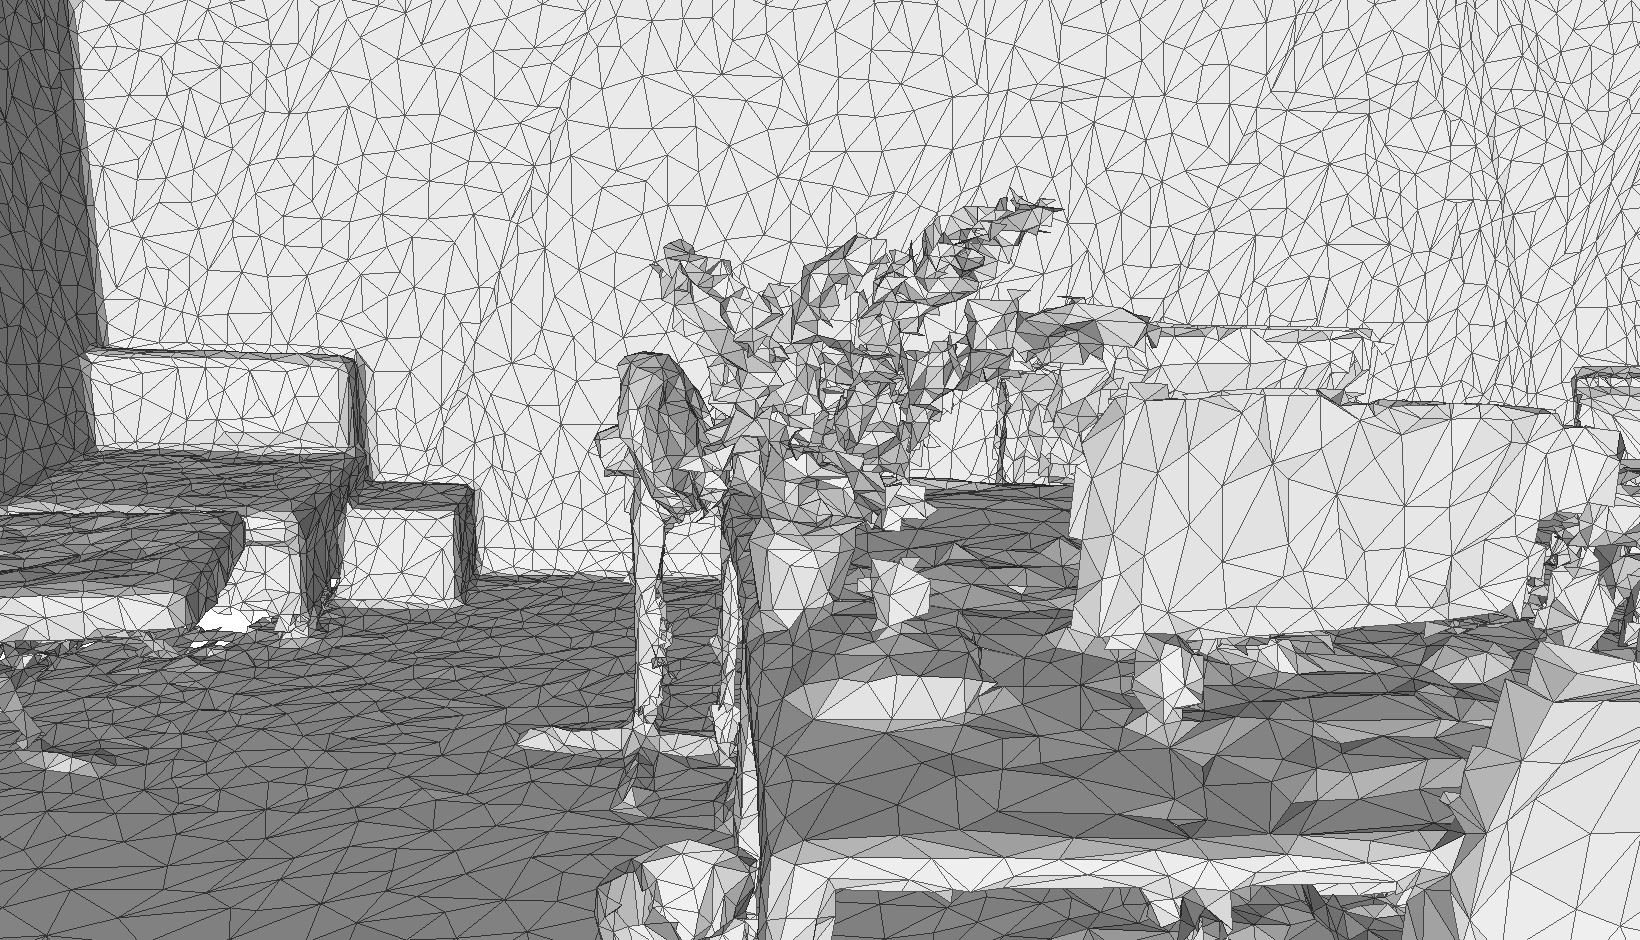
\includegraphics[width=1\textwidth]{rapid_compact}
\end{figure}
\end{frame}

\section{Questions?}
\begin{frame}
\frametitle{Questions?}
\end{frame}

\end{document}
